\documentclass{article}
\usepackage[margin=1in]{geometry}
\usepackage[numbers]{natbib}
\usepackage{graphicx}
\usepackage{amsmath}
\usepackage{amssymb}
\usepackage[parfill]{parskip} % new line between paragraphs, no indentation
\usepackage[colorlinks,pdfstartview=FitH,citecolor=blue]{hyperref}
\usepackage{xeCJK} % Enabling Chinese characters
\usepackage{fancyvrb} % In-line verbatim; for "\Verb" macro
\usepackage{float}

% Header
\usepackage{fancyhdr}
\pagestyle{fancy}
\fancyhf{}%Clear all heads and foots
\setlength{\headheight}{35pt} %Eliminate the warning of "headheight is too samll"
\rhead{Qualifying Exam Key Points\\Jianzhao Bi\\\today}
\cfoot{\thepage}

\begin{document}

\section{Aim 1}
\subsection{Key Points}
\begin{itemize}
    \item What is a convolutional layer? {
    
    A convolutional layer is computed by taking a convolutional kernel on an input layer over the entire area. The convolutional kernel function has constant parameters and can take many forms, such as mean, median or weighted averages. In a convolution layer, to obtain value of each cell, a kernel function is applied to neighboring cells and produces a scalar summary. Applying different kernel functions yields different convolutional layers. The nature of a moving average is a process of convolution. 
    \begin{equation*}
        (f*g)(t)=\int_{-\infty}^{\infty}f(\tau)g(t-\tau)d\tau
    \end{equation*}
    A convolutional layer is some form of aggregation of neighboring information for a variable. Different convolutional layers capture different levels of aggregation. Aggregation of nearby information makes it possible to capture autocorrelation. 
    }
\end{itemize}

\section{Aim 2}
\subsection{Key Points}
\begin{itemize}
    \item \textbf{Why using KED model instead of other interpolation?} {
    
    There are many other interpolation methods can be tested (such as the variational approach, that it, splines). It is necessary to check the performance of the methods, such as the preservation of geometrical properties, and then determine the final method.
    }
    \item \textbf{How to validate the qualify of the low-cost sensor calibration?} -- Cross-validation.
    \item \textbf{How to define the ``collocation'' of the AQS stations and the sensors?} {
    
    We will experiment several distances from near to far to fit the model and then use the results of cross-validation to determine which distance is the maximum threshold of the ``collocation''.
    \begin{figure}[H]
        \centering
        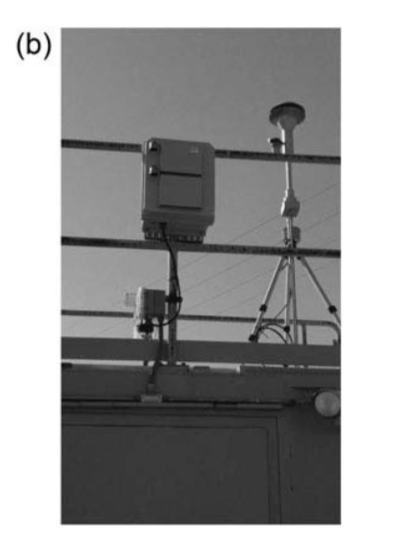
\includegraphics[width=0.35\textwidth]{img/collocation.png}
        \label{fig:col}
    \end{figure}
    }
    \item \textbf{What is PurpleAir?}
        \begin{itemize}
            \item We are a grassroots group with a technical background that wanted to measure the pollution coming from a mining operation in our backyard. The website and map was started in November 2015. Sharing the data and our research with others created a need for more monitors, to expand the network and to test the sensors by collocating them with other monitors.
            \item PurpleAir operate under an llc. We reached this point by using our own resources, some donations and help from friends.
            \item Quality techniques like an initial decay test and correlation testing with new and older monitors are used. One of the issues that faces these devices, and others, is what is called “drift”. This happens with optical particle sensors because of dust that may settle inside the device, and may cause an offset or drift over time. A maintenance schedule is necessary with any measuring device, but ours are relatively easy to maintain and cheap to service.
            \item The simplest way to view our data is the PurpleAir Map. Data is also available on MesoWest's network and others.
        \end{itemize}
        \begin{figure}[H]
            \centering
            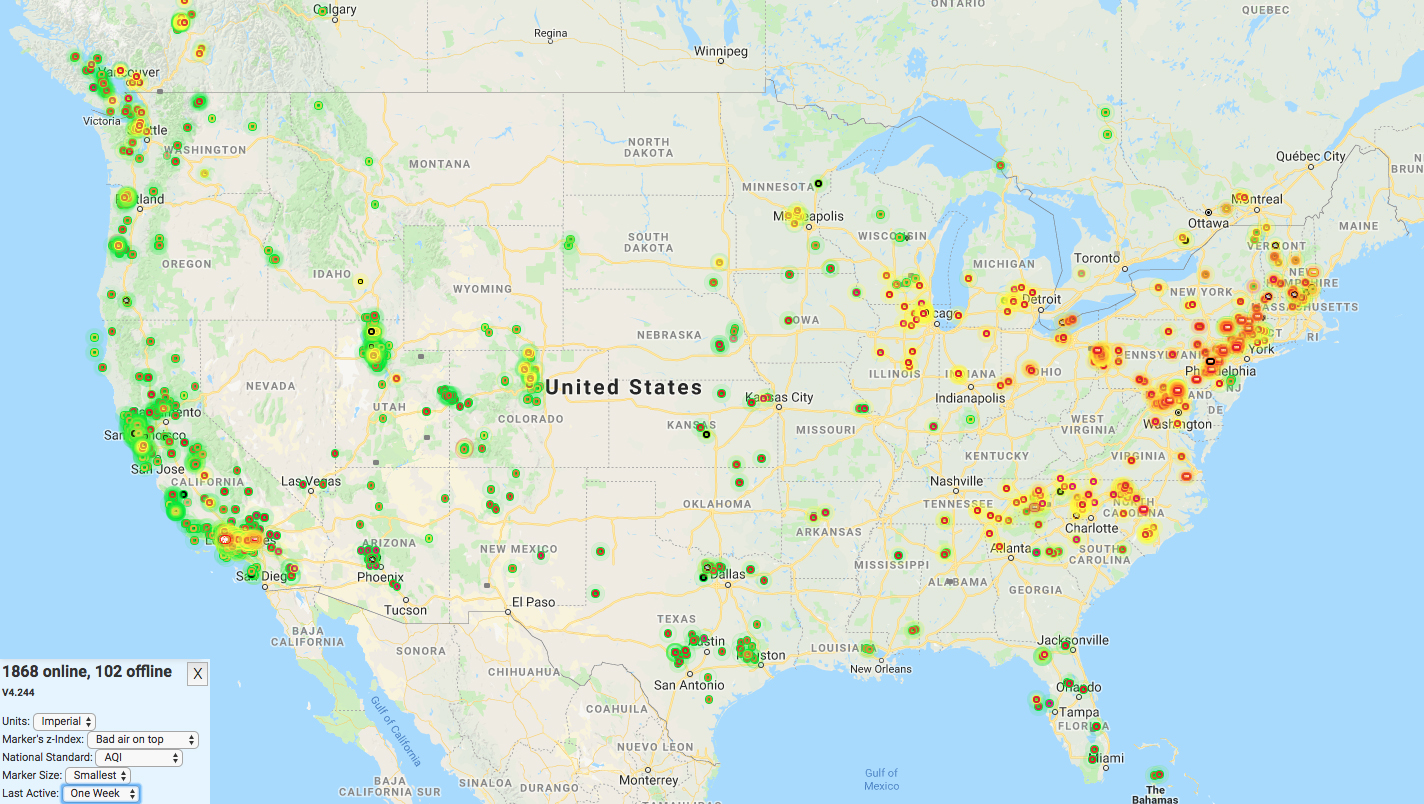
\includegraphics[width=0.8\textwidth]{img/purpleair.jpg}
            \label{fig:pa}
        \end{figure}
    \item \textbf{How do PurpleAir and FRM measurements work?} {
        \begin{itemize}
            \item \textbf{Optical light scattering/Laser counter}: PurpleAir sensors use a fan to draw air past a laser, causing reflections from any particles in the air. These reflections are used to count particles in six sizes between 0.3 $\mu m$ and 10 $\mu m$ diameter (0.3, 0.5, 1.0, 2.5, 5.0 and 10 $\mu m$). These particle counts are processed by the sensor to calculate the PM1.0, PM2.5 and PM10 mass in $\mu g/m^3$. Depending on particle composition, uncorrected measurements can vary regionally and seasonally. \citep{carvlin2017development}
            \begin{figure}[H]
                \centering
                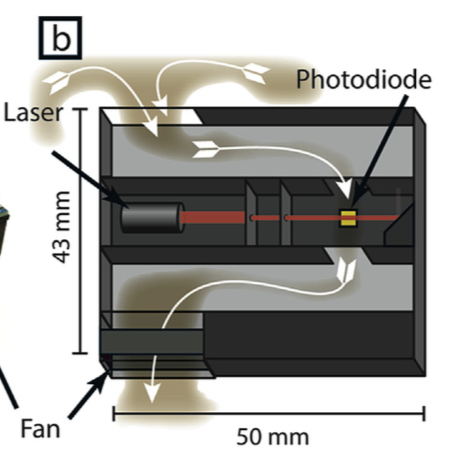
\includegraphics[width=0.3\textwidth]{img/sensor.png}
                \label{fig:sensor}
            \end{figure}
            \item \textbf{FRM/FRM}
                \begin{itemize}
                    \item Federal Reference Method: When an air pollution measurement device is designated as an FRM, this indicates it has been developed to a clearly defined standard for a specific criteria pollutant [s] and has completed a rigorous testing and analysis protocol. Successful completion of this process and designation as a ``reference method'' means that the instrument can be used to monitor compliance for the appropriate primary and/or secondary NAAQS standard for a particular criteria pollutant [s] \citep{hall2014integrating}.
                    \item Federal Equivalent Method: Air pollution measurement devices incorporating new technologies are tested and evaluated through the equivalent method process before use in the US air monitoring network. New instruments are designated as FEMs for compliance monitoring of National Ambient Air Quality Standards (NAAQS) \citep{hall2014integrating}. 
                \end{itemize}
            \item \textbf{High and low volume air samplers/Gravimetric filters (FRM)}: high and low volume air samplers are instruments used to collect samples of air particles. The difference between high and low volume air samplers is the amount of air sampled\footnote{High volume: $1500\;m^3/24\;h$; Low volume: $\leq24\;m^3/24\;h$}. Steps: 1) The inlet removes particles larger than $10 \mu m$/$2.5 \mu m$ by using their greater inertia; 2) measuring the volume of air sampled and weighing the filters before and after sampling determines the concentration of PM10/PM2.5 particles in the air.
            \item \textbf{Beta attenuation monitoring (FEM)}: BAM employs the absorption of beta radiation\footnote{Beta radiation is a high-energy, high-speed electron or positron emitted by the radioactive decay of an atomic nucleus during the process of beta decay.} by solid particles extracted from air flow. The main principle is based on a kind of Bouguer (Lambert–Beer) law: the amount by which the flow of beta radiation (electrons) is attenuated by a solid matter is exponentially dependent on its mass and not on any other feature (such as density, chemical composition or some optical or electrical properties) of this matter.
        \end{itemize}
    }
    \item \textbf{AQS PM2.5 and Sensor PM2.5} {
        \begin{itemize}
            \item If the $R^2$ between AQS PM2.5 and Sensor PM2.5 can reach 0.7, it means that two sensors have fairly good correlation, because even collocated FRM and FEM sensors only have an $R^2$ of $0.73$ with a slope of 0.66. \citep{carvlin2017development}
            \item If we cannot get the raw data (particle counts in each bin), but only estimated PM2.5 data produced by the vendor, we have to carefully consider the calibration model with extra parameters (such as meteorological variables) because the estimated PM2.5 may be fitted from these parameters. Thus, we only use polynomial model to do the calibration in the first place to avoid possible multicollinearity issues. 
            \item In a county-level study, \citet{carvlin2017development} found that there was only a marginal improvement, if any, to be gained by employing a site-specific model. 
            \item The errors between AQS and Dylos are approximately normally distributed. The calibration only makes the Dylos PM2.5 unbiased (slope = 1, intercept = 0), but does not change the correlation. There is a heteroskedasticity issue, that is, the variances of the differences become large as the PM2.5 levels become larger. In terms of the time-series, the measurements from two sensors have similar trends, indicating that the low-cost sensors can capture the pollution events.
        \end{itemize}
        \begin{figure}[H]
            \centering
            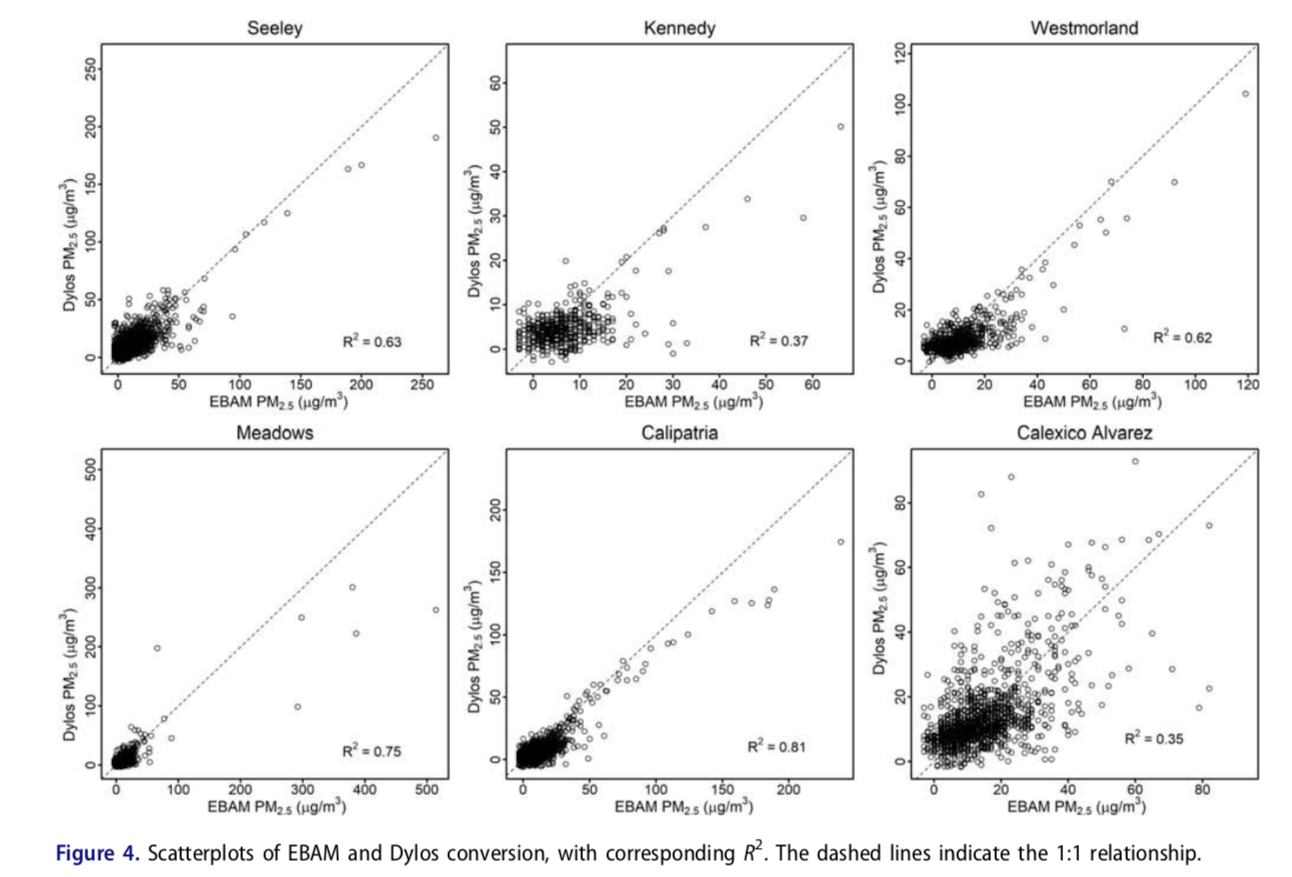
\includegraphics[width=0.8\textwidth]{img/dylos.png}
            \caption{\citet{carvlin2017development}}
            \label{fig:dylos}
        \end{figure}
        \begin{figure}[H]
            \centering
            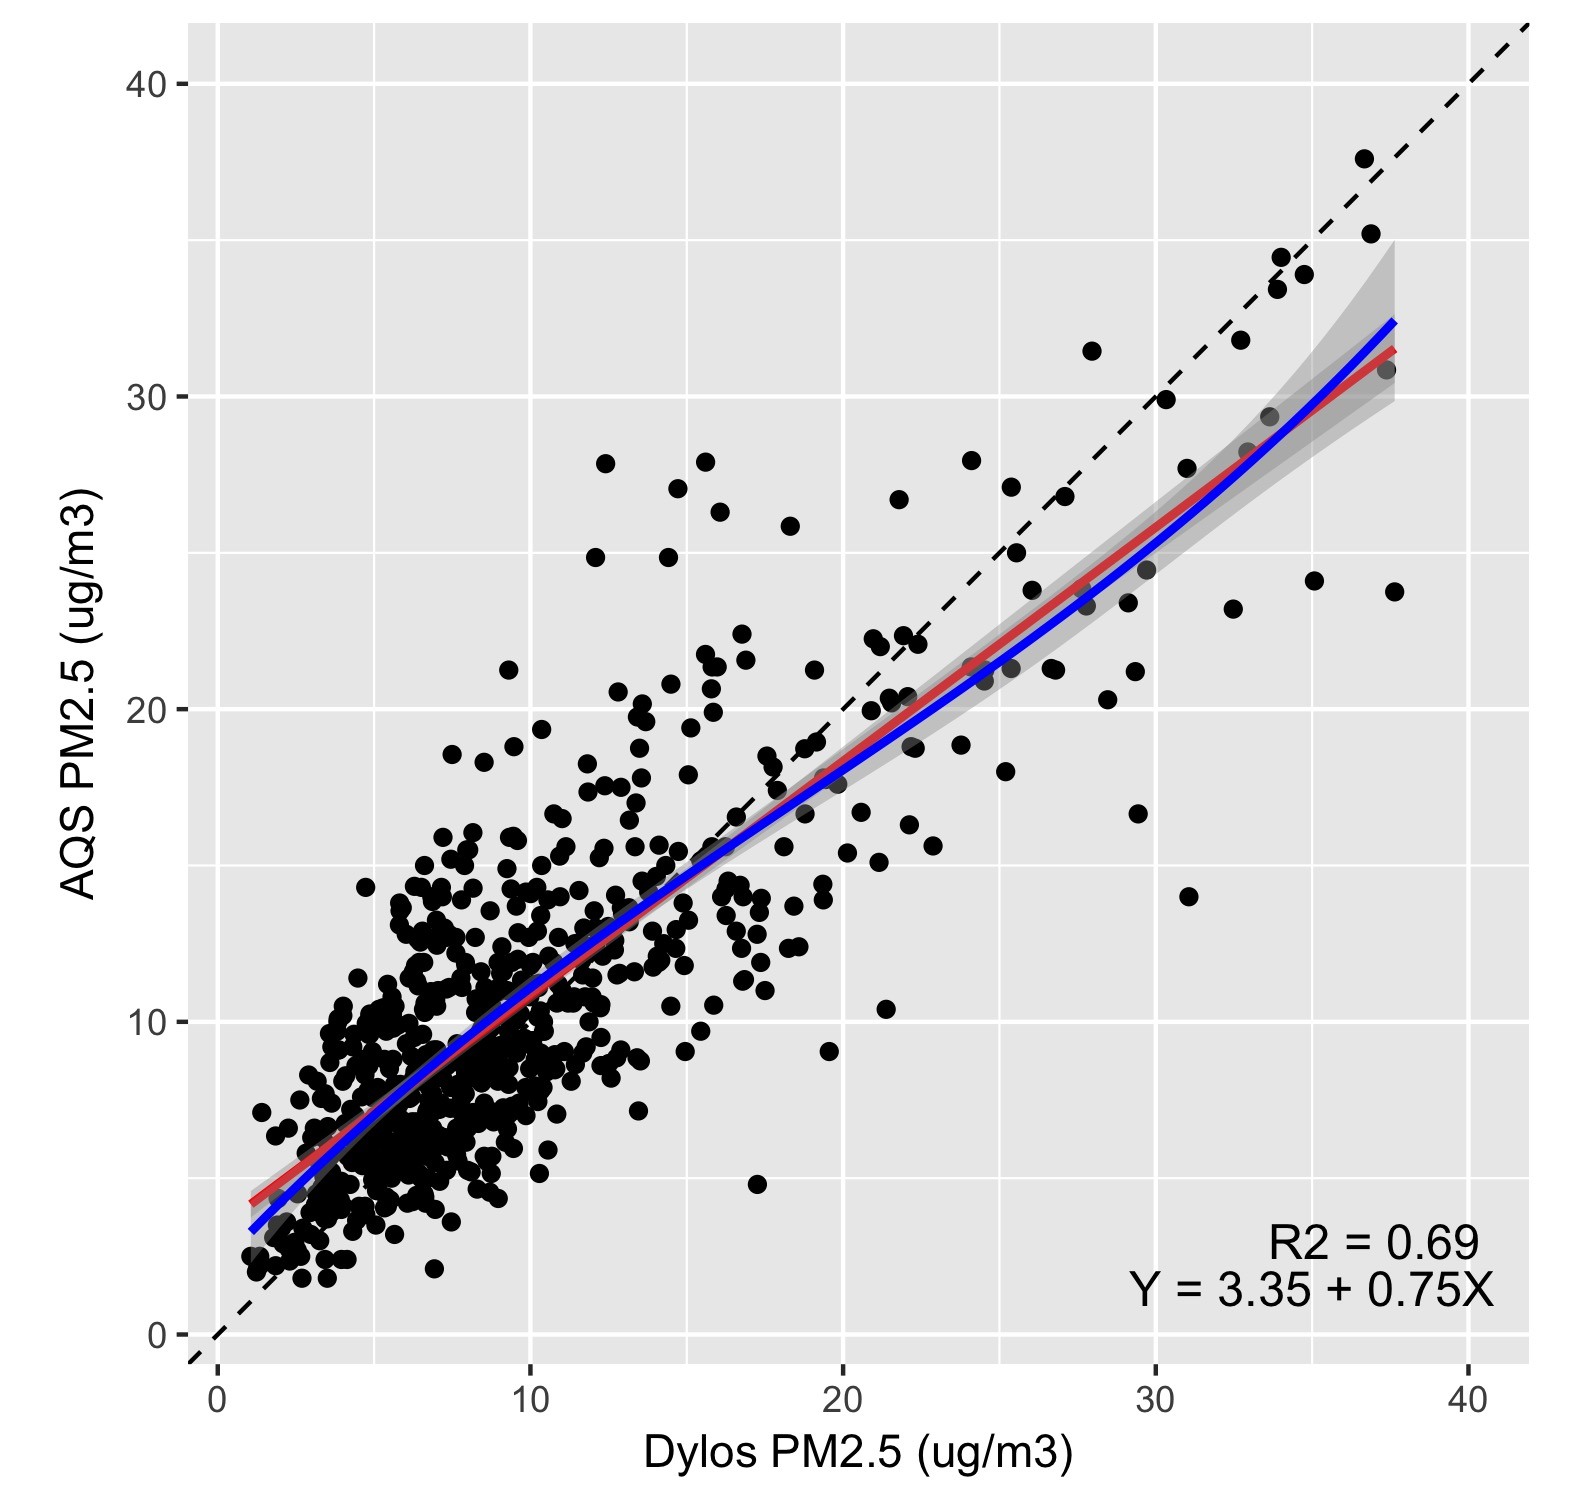
\includegraphics[width=0.45\textwidth]{img/aqs_dylos/scatter_reg.jpg} \qquad
            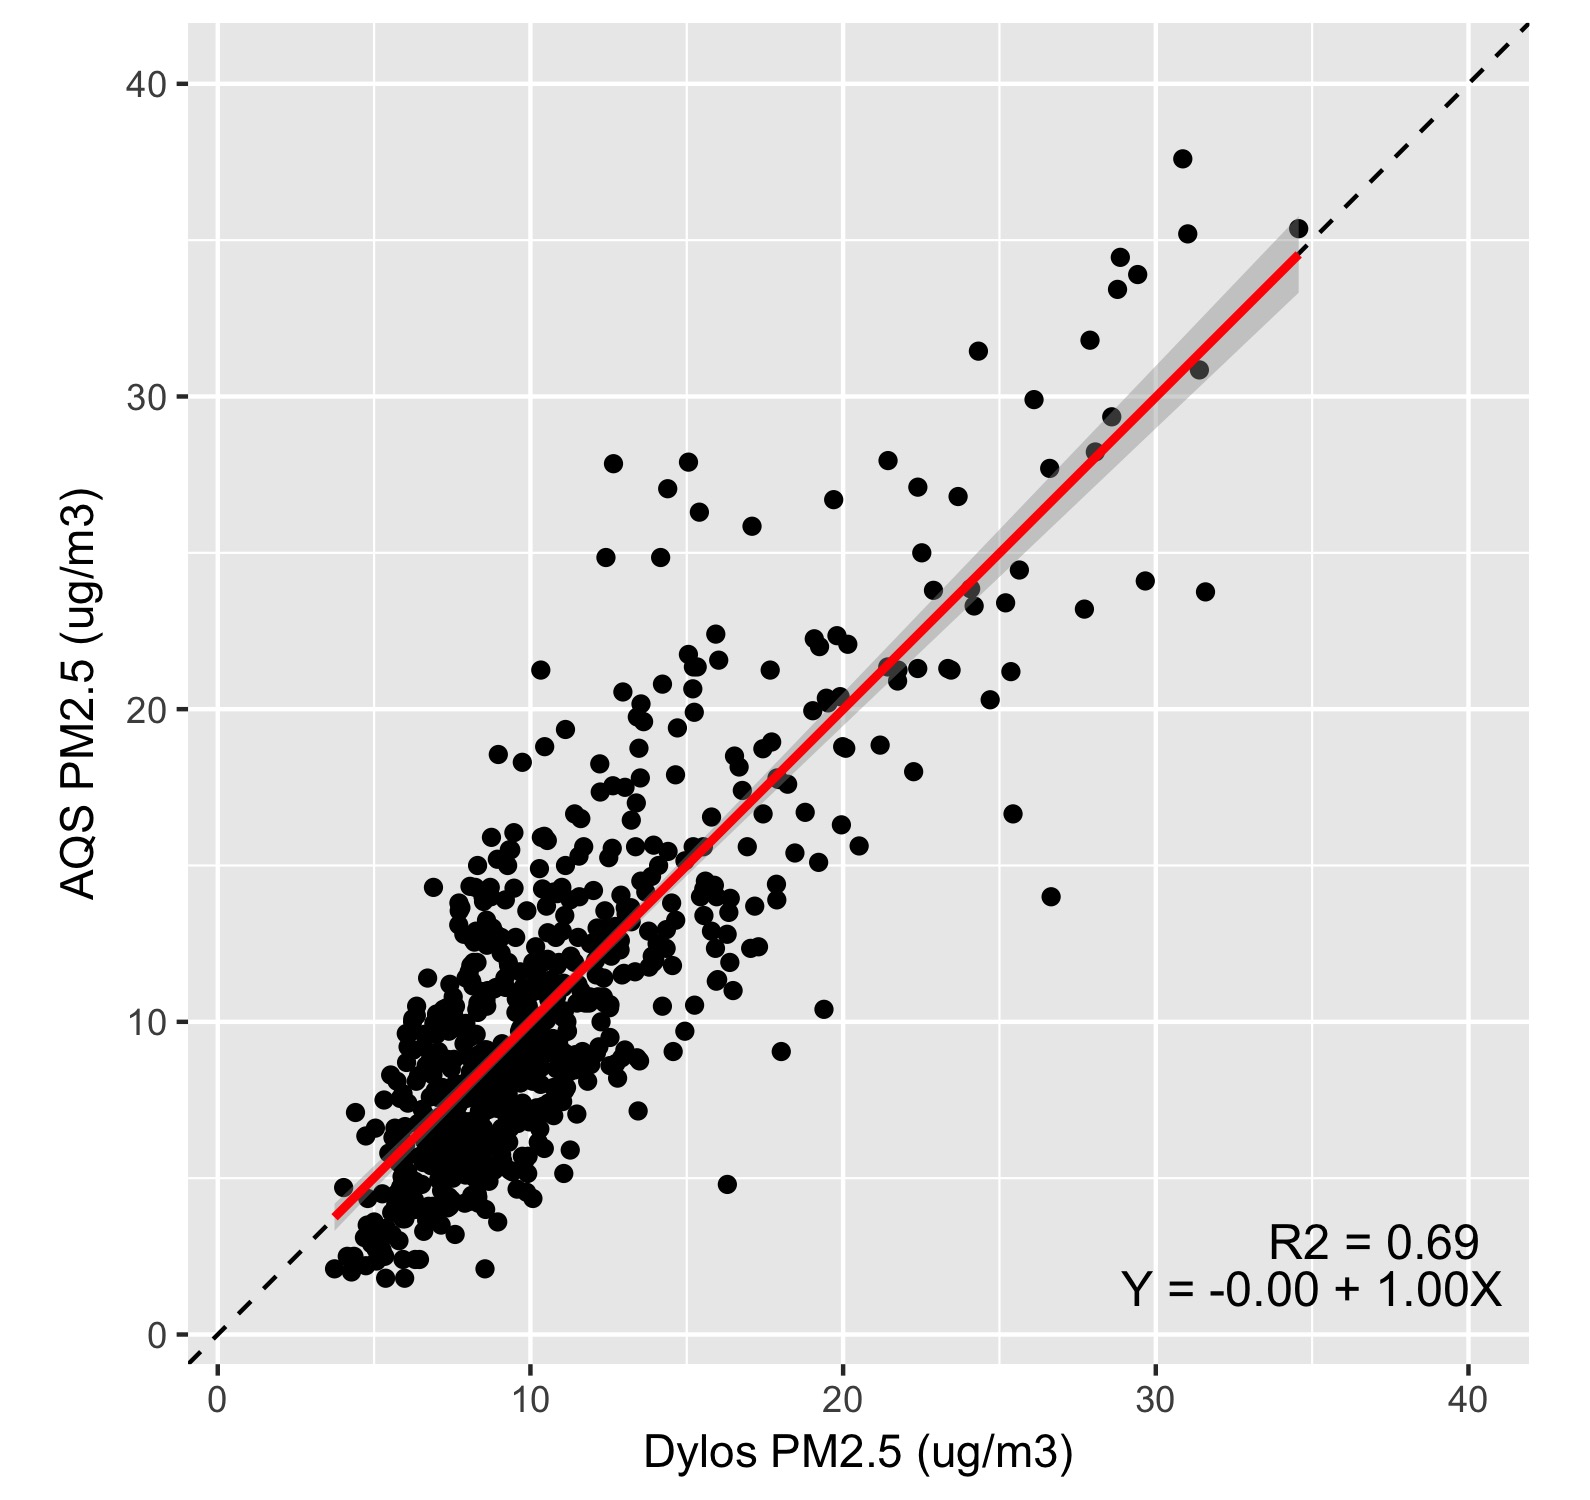
\includegraphics[width=0.45\textwidth]{img/aqs_dylos/scatter_adj.jpg}
            \caption{Left: AQS/Dylos before adjusting; Right: AQS/Dylos after adjusting}
            \label{fig:scatters}
        \end{figure}
        \begin{figure}[H]
            \centering
            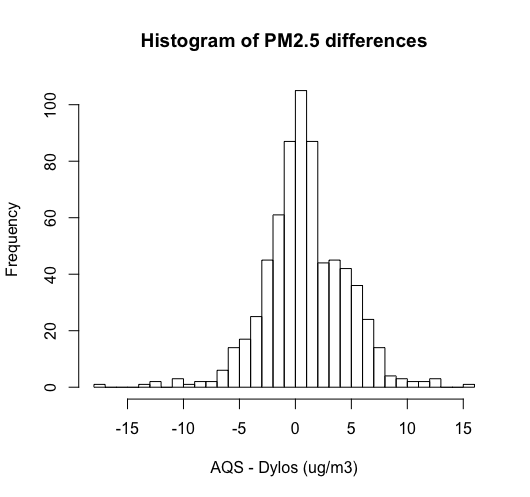
\includegraphics[width=0.45\textwidth]{img/aqs_dylos/hist.png} \qquad
            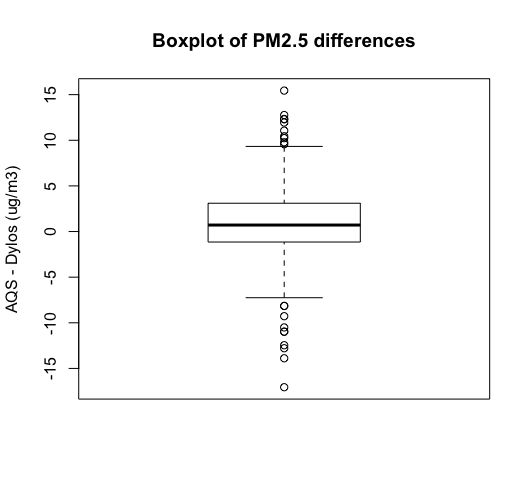
\includegraphics[width=0.45\textwidth]{img/aqs_dylos/boxplot.png}
            \caption{Left: Histogram of the difference between AQS/Dylos; Right: Boxplot of the difference between AQS/Dylos}
            \label{fig:histbox}
        \end{figure}
        \begin{figure}[H]
            \centering
            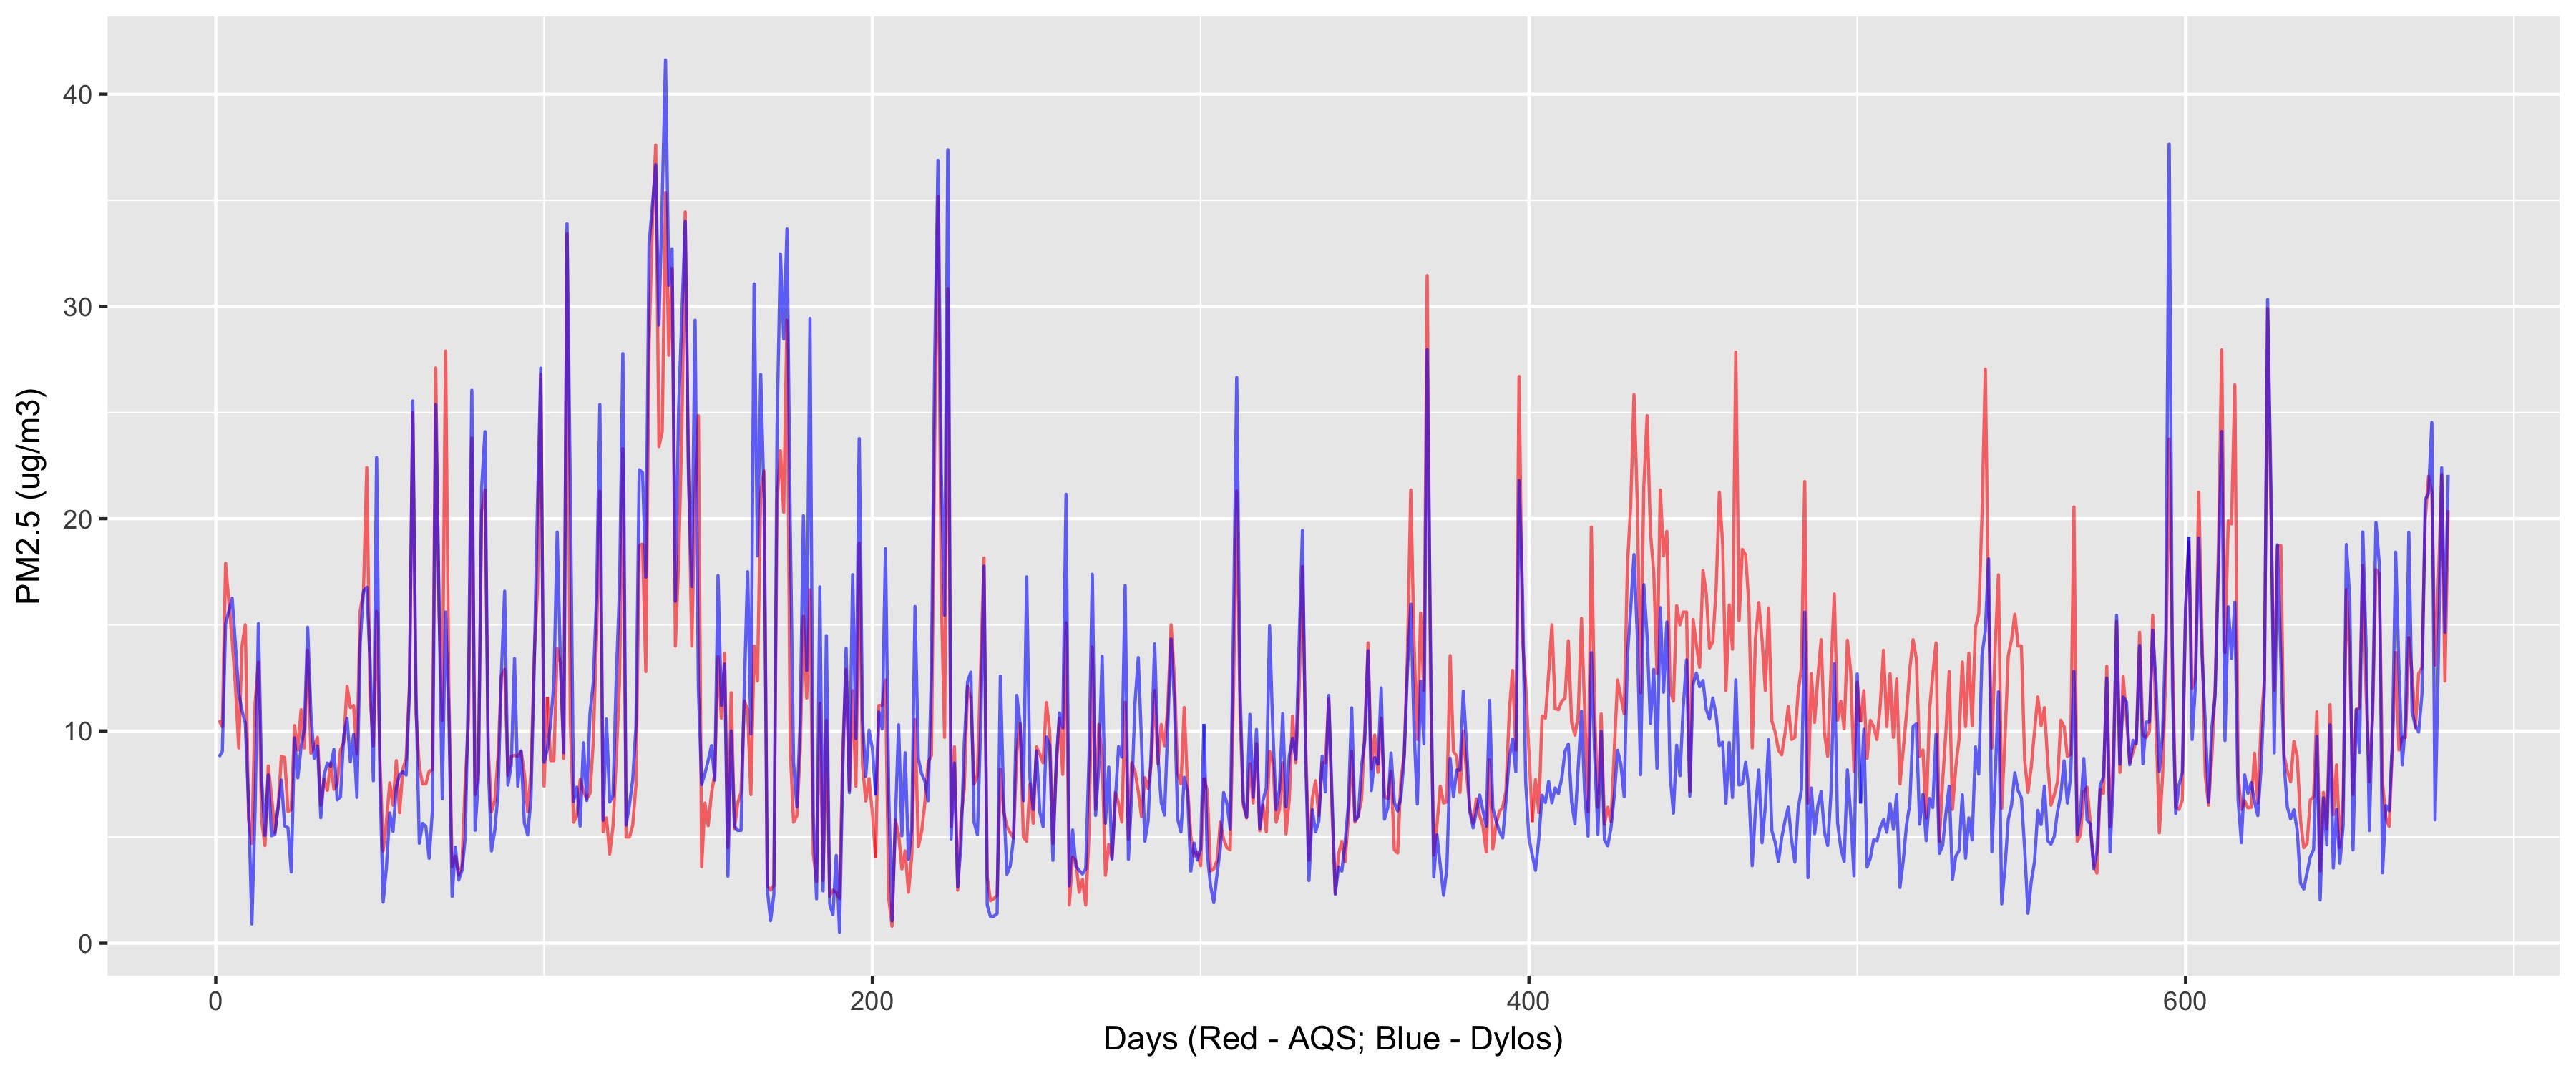
\includegraphics[width=0.9\textwidth]{img/aqs_dylos/time_series.jpg}
            \caption{Time-series for AQS/Dylos PM2.5; Red -- AQS, Blue -- Dylos}
            \label{fig:time}
        \end{figure}
    }
    
\end{itemize}

\paragraph{Related Links}
\begin{itemize}
    \item \href{http://themetoneinstrumentsmonitor.blogspot.com/2012/01/what-is-epa-designated-method.html}{What is an EPA Designated Method?}
    \item \href{https://www.qld.gov.au/environment/pollution/monitoring/air-pollution/samplers}{High and low volume air samplers}
\end{itemize}

\section{Aim 3}

\subsection{Key Points}
\begin{itemize}
    \item Routine measurements made by local and federal monitoring programs are generally available only every 3 or 6 days, which limits their usefulness for studies of associations between health outcomes and daily variations in pollutant concentrations \citep{sarnat2015fine}.
    \item Pollutants with greater measurement error are likely to exhibit weaker associations with health outcomes than pollutants with less error, even if they are not inherently less toxic.
    \item Why only choose these PM2.5 components species? {
        \begin{itemize}
            \item We selected species that represented different chemical component classes, which may plausibly confer different toxicities based on different chemical properties \citep{suh2011chemical}. 
            \item Consideration was also given to species associated with health outcomes in previous studies \citep{chen2009effects, kelly2012size, rohr2012attributing}.
            \item The concentrations of the species should be relatively high, with a small samples below the detection limit (BDL) (BDL generally $<5\%$).
        \end{itemize}
    }
    \item Covariates in the model {
        \begin{itemize}
            \item Indicator variables to control for season (\textit{i.e.,} fall, winter, spring, and summer)
            \item Day of week, holidays
            \item Time trends using cubic splines for day of visit with monthly knots (the base trend of the ED visits)
            \item Temperature: using cubic splines for lag 0 maximum temperature with knots placed at the 25$^{th}$ and 75$^{th}$ percentiles, cubic terms for 1 to 2 day moving-average minimum temperature, and cubic terms for 0 to 2 day moving-average dew point temperature \citep{strickland2010short}.
            \item \textit{\textcolor{red}{Cancer, cardiovascular disease, chronic lung disease, diabetes, hyperlipidemia (高血脂), hypertension (高血压)}}
        \end{itemize}
    }
    \item Sensitivity analysis {
        \begin{enumerate}
            \item Misspecification and the potential for residual confounding by temporal factors: estimating associations with pollutant concentrations on the day after the emergency department visit (lag $-1$) given pollutant levels on the days of interest \citep{flanders2011method}. These lag $-1$ associations are assumed to reflect noncausal mechanisms of association because the exposures occurred after the outcome, suggesting the possibility of some model misspecification and/or residual confounding in primary models assessing the effects of these pollutants \citep{flanders2011method}.
            \item Alternate model specifications: 1) alternate time trend control (cubic spline for day of visit with two knots per month and one knot every 2 months, respectively, instead of one knot per month); 2) alternate temperature control (indicator variables for each degree Celsius instead of a cubic spline for lag 0 maximum temperature).
            \item Assess the robustness of our results to lag structure: examined 5-day distributed lag models (lags 0--4), with control for minimum and dew point temperature adjusted to include the moving average of lags 1--4 and 0--4, respectively.
            \item Potential for confounding of selected single-pollutant results: co-pollutants using two-pollutant models
        \end{enumerate}
    }
    \item How to estimate the burden of kidney disease caused by PM2.5 exposure? {
        \begin{itemize}
            \item Population attributable fraction (PAF) represents the proportional reduction in population disease that would occur if exposure to PM2.5 was reduced to the Environmental Protection Agency's (EPA) recommended levels of 12 $mg/m^3$ \citep{bowe2018particulate}.
            \item \citet{bowe2018particulate} estimated the national burden of CKD attributable to elevated levels of PM2.5 exceeding the EPA standard (where the theoretical minimum risk exposure level [TMREL] was set at the EPA standard of 12 $mg/m^3$) in the contiguous United States was 44,793 incident cases per year (95\% uncertainty interval [95\% UI], 42,716 to 46,869). The national burden of ESRD attributable to PM2.5 levels in excess of EPA standards was 2438 incident cases per year (95\% UI, 1963 to 2902). 
        \end{itemize}
    }
    \item \href{https://rdrr.io/cran/powerMediation/man/sizePoisson.html}{Sample size} calculation for simple Poisson regression. Assume the predictor is normally distributed. {
       
        Take PM2.5 as an example: the mean concentration is $15\;\mu g/m^3$; the standard deviation is $7\;\mu g/m^3$; the IQR is $9\;\mu g/m^3$; the expected rate ratio is 1.035; Then, according to ``\Verb+sizePossion+'', the minimum sample size is 8741 counts at 5\% significance level and the power of 0.8. If the average daily counts for ARF is 10 $person/day$, there should be 874 days' data ($\sim 2.4\;years$). 
         \begin{verbatim}
            library(powerMediation)
            sizePoisson(beta0 = 0, beta1 = log(1.035)/9, mu.x1 = 15, 
                sigma2.x1 = 7*7, mu.T = 1, phi = 1, alpha = 0.1, power = 0.8)
        \end{verbatim}
    }
    \fbox{
        \parbox{0.9\textwidth}{
            The simple Poisson regression has the following form:
            \begin{equation*}
                Pr(Y_i = y_i | \mu_i, t_i) = \exp(-\mu_i t_i) (\mu_i t_i)^{y_i}/ (y_i!)
            \end{equation*}
            where
            \begin{equation*}
                \mu_i=\exp(\beta_0+\beta_1 x_{1i})
            \end{equation*}
            We are interested in testing the null hypothesis $\beta_1=0$ versus the alternative hypothesis $\beta_1=\theta_1$. Assume $x_1$ is normally distributed with mean $\mu_{x_1}$ and variance $\sigma^2_{x_1}$. The sample size calculation formula derived by \citet{signorini1991sample} is
            \begin{equation*}
                N=\phi{[z_{1-\alpha/2}\sqrt{V(b_1 | \beta_1=0)} +z_{power}\sqrt{V(b_1 | \beta_1=\theta_1)}]^2}/ {\mu_T \exp(\beta_0) \theta_1^2}
            \end{equation*}
            where $\phi$ is the over-dispersion parameter $(var(y_i)/mean(y_i))$, $\alpha$ is the type I error rate, $b_1$ is the estimate of the slope $\beta_1$, $\beta_0$ is the intercept, $\mu_T$ is the mean exposure time, $z_a$ is the $100\times\alpha^{th}$ lower percentile of the standard normal distribution, and $V(b_1|\beta_1=\theta)$ is the variance of the estimate $b_1$ given the true slope $\beta_1=\theta$.
            
            The variances are
            \begin{equation*}
                V(b_1 | \beta_1 = 0)=1/{\sigma^2_{x_1}}
            \end{equation*}
            and
            \begin{equation*}
                V(b_1 | \beta_1 = \theta_1)=1/{\sigma^2_{x_1}} \exp[-(\theta_1 \mu_{x_1} + \theta_1^2\sigma^2_{x_1}/2)]
            \end{equation*}
        }
    }
\end{itemize}

\subsection{Statistical Knowledge}
\begin{itemize}
    \item Standardization is the necessary step for the hypothesis testing, that is, to transform a specific distribution to its standard distribution (\textit{e.g.,} standard normal distribution $z=\frac{X-\mu}{\sigma}$). By doing this, the probability can be easily calculated. 
    \item IQR is more robust (less sensitive) than Range. IQR is not as sensitive to shape of distribution or to extreme values (outliers).
    \item Confidence Interval (CI): a level $C=1-\alpha$ confidence interval for a parameter is an interval computed from sample data by a method that has probability $C$ of producing an interval containing the true value of the parameter.
        \begin{itemize}
            \item The observed interval brackets the true value of $\mu$, with confidence $100(1-\alpha)\%$; that is the procedure successfully yields a CI that captures the true value $100(1-\alpha)\%$ of the time. 
            \item With repeated sampling, $100(1-\alpha)\%$ of the intervals formed using this procedure will capture the true value of $\mu$.
        \end{itemize}
         \begin{align*}
                   &P[-z_{\alpha/2}\leq \frac{\bar{X}-\mu}{\sigma/\sqrt{n}}\leq z_{\alpha/2}]=1-\alpha \\
        \therefore &P[\bar{X}-z_{\alpha/2}\frac{\sigma}{\sqrt{n}}\leq \mu \leq \bar{X}+z_{\alpha/2}\frac{\sigma}{\sqrt{n}}]=1-\alpha
        \end{align*}
\end{itemize}

\bibliographystyle{plainnat}
\bibliography{references}

\end{document}